% Generated by render.py; edit preamble.tex and equality.tikz
\documentclass[border=12pt]{standalone}
\def\pgfsysdriver{pgfsys-dvisvgm.def}
\usepackage[dvisvgm]{xcolor}
\usepackage{xeCJK}
\setCJKmainfont{HaranoAjiGothic-Regular.otf}[BoldFont=HaranoAjiGothic-Bold.otf]
\setCJKsansfont{HaranoAjiGothic-Regular.otf}[BoldFont=HaranoAjiGothic-Bold.otf]
\usepackage{amsmath,amssymb,tikz,lmodern}
\usetikzlibrary{arrows.meta,positioning,calc,fit,backgrounds}
\renewcommand{\familydefault}{\sfdefault}
\definecolor{ink}{HTML}{25322F}
\definecolor{green}{HTML}{246657}
\definecolor{tint}{HTML}{EEF4F0}
\definecolor{soft}{HTML}{C6D2CC}
\definecolor{muted}{HTML}{52615B}
\newif\ifJapanese
\newcommand{\Tx}[2]{\ifJapanese #1\else #2\fi}
\newcommand{\Eff}{\overline{\operatorname{Eff}}}
\newcommand{\heading}[3]{{\color{green}\bfseries #1\quad\Tx{#2}{#3}}\\[5pt]}
% A white rectangle makes the complete citation label clickable, including spaces.
\newcommand{\refurl}[2]{\special{dvisvgm:raw <a xlink:href="#1" target="_blank" rel="noopener noreferrer">}{\setlength{\fboxsep}{0pt}\colorbox{white}{\color{green}\underline{\strut #2}}}\special{dvisvgm:raw </a>}}
\tikzset{
 card/.style={draw=soft,fill=white,rounded corners=2pt,align=left,text=ink,font=\fontsize{10.5}{14}\selectfont,inner xsep=12pt,inner ysep=10pt,text width=14.4cm},
 half/.style={card,text width=6.45cm,minimum height=2.05cm},
 result/.style={card,draw=green,fill=tint,line width=.9pt},
 reason/.style={align=left,text=muted,font=\fontsize{9}{12}\selectfont,inner sep=0pt,text width=12.6cm},
 branchreason/.style={reason,text width=5.95cm},
 edge/.style={-{Stealth[length=2.4mm]},draw=green,line width=1pt},
 wire/.style={draw=green,line width=1pt},
}
% Keep the arrow in a dedicated left gutter; explanations never cover it.
\def\flow#1#2#3;{
 \coordinate (#2-from) at ($(#1.south)+(-6.9,0)$);
 \coordinate (#2-to) at ($(#2.north)+(-6.9,0)$);
 \draw[edge] (#2-from)--(#2-to);
 \node[reason,anchor=west] (#2-reason) at ($(#2-from)!.5!(#2-to)+(.55,0)$) {#3};
}

% Style adapted from the repository's Schnell diagrams; MIT attribution retained.
\newcommand{\PRef}[1]{\refurl{https://github.com/openai/math/blob/fd4aeeb2ee4fc729c18d98444fed42fd0529eeeb/preprints/The-Generalized-Mukai-Conjecture-September-24-2026/article.pdf}{#1}}
\newcommand{\MMRef}[1]{\refurl{https://arxiv.org/pdf/math/0409569v4\string##page=5}{#1}}
\newcommand{\TZRef}[1]{\refurl{https://arxiv.org/pdf/1209.4342v5\string##page=4}{#1}}
\newcommand{\KMRef}[1]{\refurl{https://www.ihes.fr/~maxim/TEXTS/relation_between_23.pdf\string##page=7}{#1}}
\newcommand{\PARef}[1]{\refurl{https://www.numdam.org/item/SB_1997-1998__40__307_0.pdf\string##page=6}{#1}}
\newcommand{\BCRef}[1]{\refurl{https://druel.perso.math.cnrs.fr/textes/mukai.pdf\string##page=23}{#1}}
\newcommand{\ERRef}[1]{\refurl{https://druel.perso.math.cnrs.fr/textes/mukai_erratum.pdf}{#1}}
\newcommand{\OCRef}[1]{\refurl{https://doi.org/10.4153/CMB-2006-028-3}{#1}}

\Japanesefalse
\begin{document}
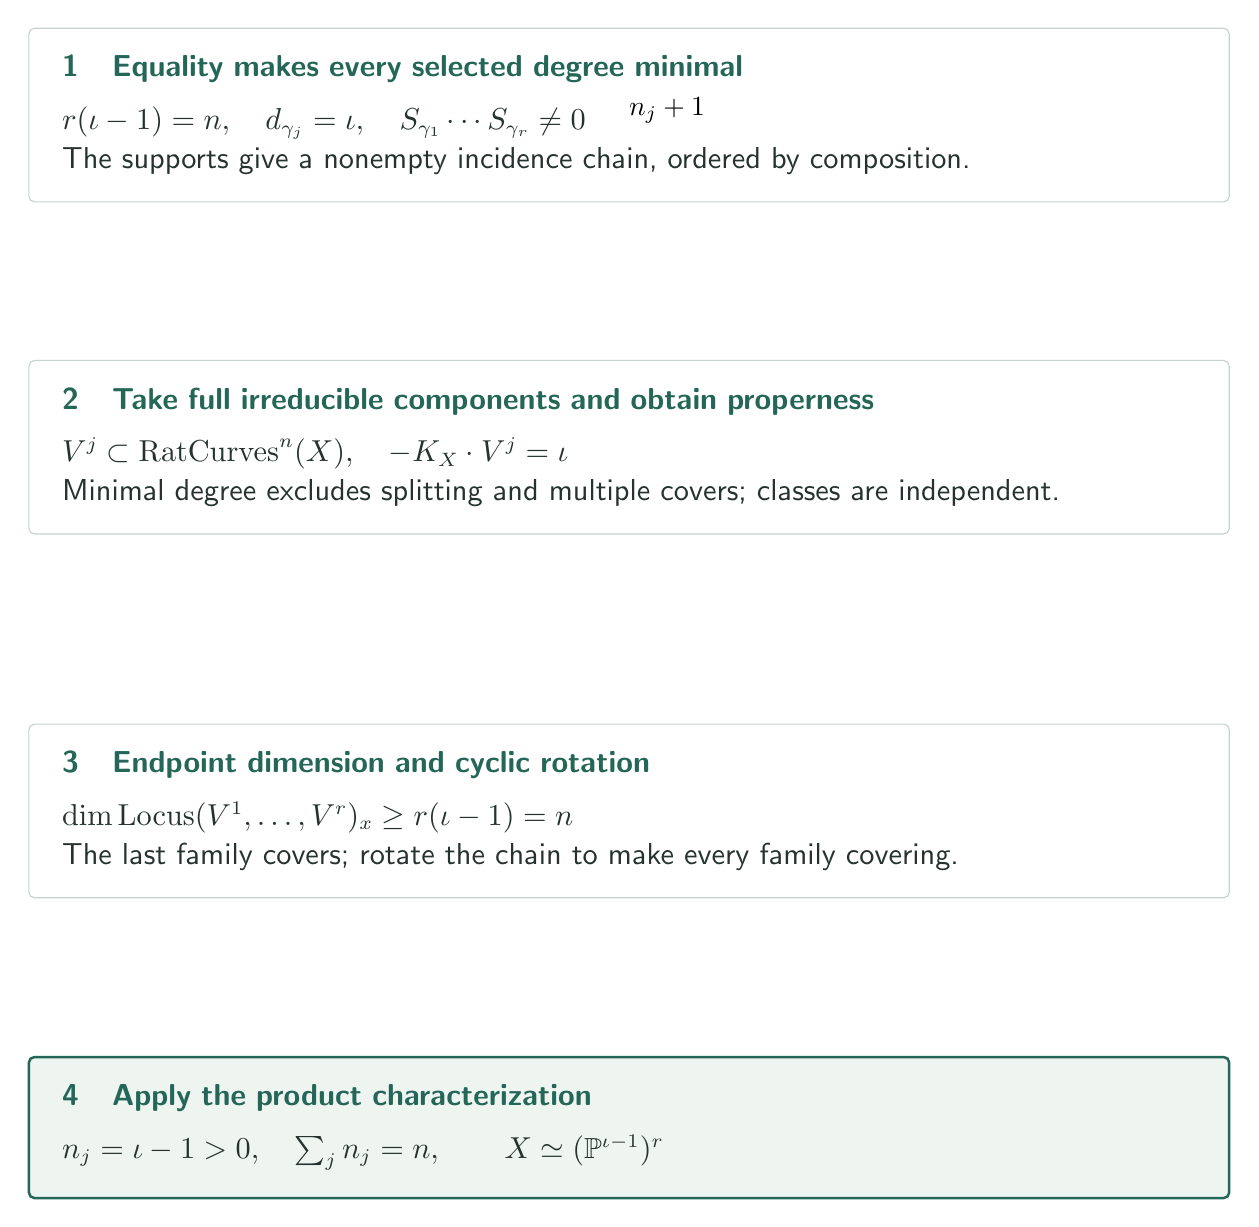
\begin{tikzpicture}

\node[card] (a) {\heading{1}{等号がすべての曲線次数を最小にする}{Equality makes every selected degree minimal}
$r(\iota-1)=n,\quad d_{\gamma_j}=\iota,\quad
S_{\gamma_1}\cdots S_{\gamma_r}\ne0$\\
\Tx{対応の台から、合成順に沿う非空な incidence chain を得る}{The supports give a nonempty incidence chain, ordered by composition.}};
\node[card,below=2cm of a] (b) {\heading{2}{全既約成分を取って proper 性を得る}{Take full irreducible components and obtain properness}
$V^j\subset\mathrm{RatCurves}^{n}(X),\quad -K_X\cdot V^j=\iota$\\
\Tx{最小次数により分裂・多重被覆を排除。数値類は独立}{Minimal degree excludes splitting and multiple covers; classes are independent.}};
\flow{a}{b}{\Tx{評価像の台、最小次数の安定極限を使用：}{Use the evaluation supports and stable limits of minimal degree:}\\
\PRef{Lemma 6.3, pp. 16--17}\quad\Tx{任意の部分族ではなく全成分を選ぶ}{Choose full components, not arbitrary subfamilies.}};
\node[card,below=2.4cm of b] (c) {\heading{3}{endpoint の次元評価と巡回操作}{Endpoint dimension and cyclic rotation}
$\dim\mathrm{Locus}(V^1,\ldots,V^r)_x\ge r(\iota-1)=n$\\
\Tx{最後の族が covering。chain を巡回させ、すべての族を covering にする}{The last family covers; rotate the chain to make every family covering.}};
\flow{b}{c}{\BCRef{Mukai chain bound, Thm. 5.2, p. 623}\ +\ \ERRef{Erratum, p. 1}\\
\Tx{訂正の「proper な既約成分」という仮定を確認：}{The corrected hypothesis requires proper irreducible components:}\\
\PRef{Thm. 6.1; Prop. 6.4, pp. 16--17}};
\node[result,below=2cm of c] (d) {\heading{4}{積の特徴付けを適用}{Apply the product characterization}
$n_j=\iota-1>0,\quad \sum_j n_j=n,\qquad
X\simeq(\mathbb P^{\iota-1})^r$};
\flow{c}{d}{\Tx{unsplit・covering・独立な族と次数 $n_j+1$ が揃う：}{Unsplit, covering, independent families have degrees $n_j+1$:}\\
\OCRef{Product characterization, Thm. 1.1, p. 271}\quad \PRef{Prop. 6.4, p. 17}};

\end{tikzpicture}
\end{document}
